\chapter{Podsumowanie, możliwe drogi dalszych badań}\label{chap:results_analysis}


Wyniki przedstawione w rozdziałach~\ref{chap:research} oraz~\ref{target_function_chapter}
wskazują, że zaimplementowany algorytm optymalizacji wytwarza poprawne rozwiązania
dla prostych problemów, przedstawionych w sekcji~\ref{sec:predefined_graph_optimisation},
jednak nie potrafi odtworzyć bardziej złozonych dźwięków -- w porównaniu
wypada gorzej niż algorytm z literatury~\cite{evolutionary_puredata}.
Testy wykonane w rozdziale~\ref{target_function_chapter} pokazują,
że zaproponowana w pracy funkcja celu prowadzi do udanej optymalizacji
struktury i parametrów grafu dla prostych wariantów problemów.
Wygenerowane struktury grafu opisane w rozdziale~\ref{chap:research} pokazują
poprawnie odtworzone węzły DSP typowe dla syntezy, która powinna zostać
wykorzystana do wytworzenia konkretnych rodzajów dźwięków.

% Nawet gdy finalnie wygenerowane brzmienie różni się od dźwięku docelowego,
% algorytm wytwarza interesujące barwy dźwięku,
% które można zakwalifikować jako~,,wariacje'' na temat oryginalnego sygnału.
% Tego typu wyniki mogą być wartościowe dla potencjalnych użytkowników algorytmu.
% W niniejszym rozdziale przeprowadzono szczegółową analizę obserwacji,
% uzyskanych podczas procesu badawaczego.


\section{Zbiór danych testowych}\label{sec:not_enough_benchmarking_data}

Automatyczna konstrukcja elektronicznych instrumentów muzycznych jest stosunkowo
nowym obszarem badań, w związku z czym brakuje odpowiednich zbiorów danych
umożliwiających porównywanie sprawności różnych algorytmów.
Porównanie wykonane w niniejszej pracy nie stanowi przekroju
przez wiele możliwych typów syntezy, ponieważ w procesie przeglądu
literatury nie udało się znaleźć stosownego zbioru danych.

Jak pokazały wyniki opisane w sekcji~\ref{sec:non_literature_samples},
zaimplementowany algorytm generuje lepsze rozwiązania w przypadku
syntezy \textit{analog modeling}, podczas gdy praca służąca
za porównanie~\cite{evolutionary_puredata} zawiera głownie dźwięki wytworzone
za pomocą syntezy FM oraz nagrania instrumentów dętych.


\section{Potencjał wykorzystania w przemyśle muzycznym}\label{sec:music_industry_usage}

Wytwarzane przez algorytm barwy są zróżnicowane i brzmią
w sposób~,,muzyczny'' -- nawet gdy wygenerowany dźwięk
znacząco różni się od docelowej barwy, algorytm nie generuje
szumu ani~,,kakofonii''. 
Zaimplementowany algorytm może być uruchomiony na standardowym komputerze,
dostępnym dla przeciętnego użytkownika, co otwiera możliwość jego integracji
z oprogramowaniem typu \textit{digital audio workstation}. Integracja
z oprogramowaniem do produkcji muzyki otwiera drogę do wykorzystania
wtyczek \texttt{VST}, znacznie zwiększając liczbę dostępnych
dla algorytmu węzłów przetwarzania sygnału, potencjalnie usprawniając
jego działanie. Proponowanym środowiskiem, które można wykorzystać w celu zintegrowania
zaimplementowanego algorytmu z oprogramowaniem \textit{digital audio workstation}
i wtyczkami w technologii \texttt{VST} jest program
\texttt{DawDreamer}~(\url{https://github.com/DBraun/DawDreamer}).


\section{Potencjalne usprawnienia wydajności algorytmu}

Rysunki~\ref{fig:target_function_profiling} oraz~\ref{fig:mfcc_profiling}
przedstawiają wyniki profilowania zaimplementowanego algorytmu, wykonane
za pomocą narzędzia \href{https://jiffyclub.github.io/snakeviz/}{\texttt{snakeviz}}.
W pracy została wykorzystana gotowa implementacja
algorytmu DTW (\textit{dynamic time warping}) w języku \texttt{Python}, której
wykonanie zajmuje największą część czasu obliczania wartości funkcji celu.
Wykorzystanie pakietu numerycznego \texttt{numpy} bądź implementacja DTW w
kompilowanym języku programowania może znacząco poprawić szybkość działania algorytmu.

\begin{figure}[H]
    \centering
    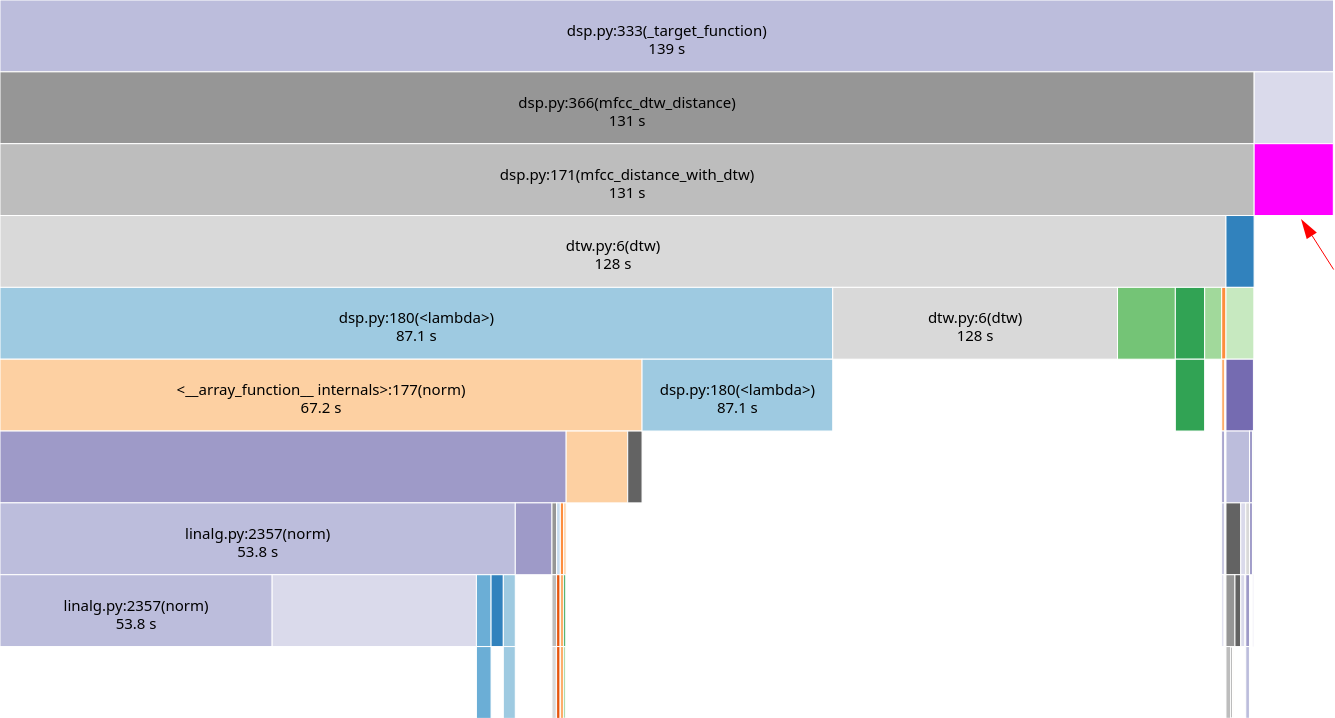
\includegraphics[width=1.0\linewidth]{rys07/profile_target_function_execution.png}
    \caption{
      Wizualizacja danych wygenerowanych przez profiler języka Python
      dla przykładowego problemu optymalizacji. Widoczne składowe wpływające
      na sumaryczny czas ewaluacji funkcji celu.
      Czerwoną strzałką oznaczono czas poświęcony
      na syntezę dźwięku w grafie DSP\@.
    }\label{fig:target_function_profiling}
\end{figure}

\begin{figure}[H]
    \centering
    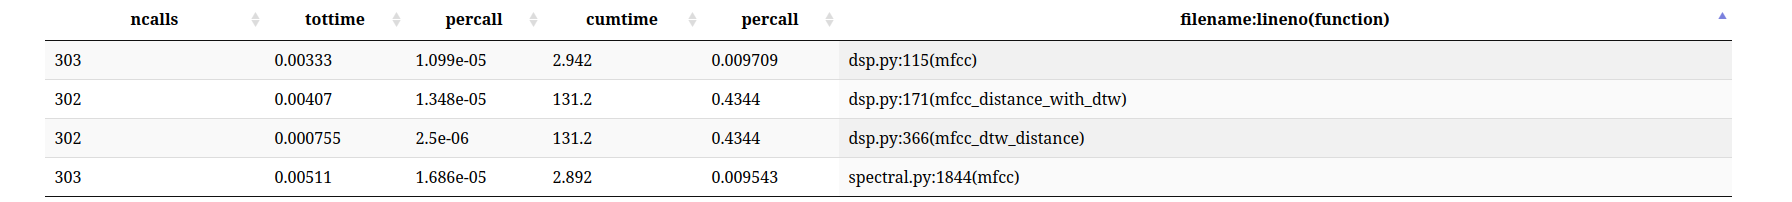
\includegraphics[width=1.0\linewidth]{rys07/mfcc_search.png}
    \caption{
      Porównanie czasu obliczania współczynników MFCC (\texttt{dsp.py:115})
      oraz czasu działania algorytmu DTW (\texttt{dsp.py:171}).
    }\label{fig:mfcc_profiling}
\end{figure}


\section{Potencjalne drogi dalszego rozwoju algorytmu}\label{sec:potential_improvements}

\subsection{Rozmiar okna w algorytmie DTW}

W domyślnym wariancie, algorytm DTW przeszukuje cały sygnał
przy poszukuwaniu pasujących do siebie segmentów. Takie
zachowanie zwiększa złożoność czasową algorytmu, jednocześnie
zmniejszając karę za niedokładne odwzorowanie zmian w dynamice dźwięku.
Przeprowadzone w ramach pracy testy pozwalają wnioskować, że zmniejszenie
rozmiaru okna w algorytmie DTW pozwoli na skrócenie czasu
wyliczania funkcji celu i jednocześnie usprawni wyniki optymalizacji
w zakresie dokładności odwzorowania dynamiki dźwięku.

  % \item Różne wielkości okna DTW,
\subsection{Lepsza reprezentacja struktury grafu DSP w genotypie}

Jak opisano w sekcji~\ref{sec:graph_structure_definition}, genotyp grafu DSP
podzielony jest na dwa fragmenty:

\begin{itemize}
  \item $S$ -- fragment odpowiadający za strukturę grafu,
  \item $P$ -- fragment odpowiadający za wartości parametrów w grafie.
\end{itemize}

Po wygenerowaniu danej struktury grafu $G_s$~(\ref{eq:graph_structure_generation_function}),
parametry grafu przypisywane są poprzez równoczesne iterowanie przez wektor $P$ oraz
przez listę parametrów w wygenerowanym grafie $G_s$. Zastosowanie takiego algorytmu
powoduje, że zmiana struktury grafu może spowodować przypisanie parametrów w inne miejsca
na nowym grafie, gdzie ich wartości będą miały zupełnie inny wpływ na sygnał
generowany przez graf. Problem można rozwiązać poprzez trwałe przypisanie danych
parametrów $p_i$ do konkretnych parametrów konkretnej struktury w grafie. Jeśli gen 
tworzący daną strukturę nie będzie aktywny, geny określające parametry tej struktury nie będą
miały wpływu na generowany sygnał i nie zaburzą sposobu przypisania pozostałych genów.


\subsection{Dalsze poszukiwania funkcji celu porównującej barwę sygnałów dźwiękowych}

W pracach przeanalizowanych podczas przeglądu literatury wykorzystano 2 podejścia
do porównania barwy sygnałów dźwiękowych: różnica między spektrogramami oraz
różnica między wartościami współczynników MFCC
(szczegóły opisano w rozdziale~\ref{target_function_chapter}).
Wyniki przeglądu literatury pozwalają podejrzewać, że porównywanie sygnałów
dźwiękowych pod względem ich barwy w kontekście brzmienia muzycznego
nie jest szeroko zbadanym problemem i istnieje potencjał na opracowanie
nowych rozwiązań.


\subsection{Rozszerzenie genotypu grafu DSP o dodatkowe źródła modulacji}

W syntezatorach dźwięku często wykorzystuje się sygnały modulujące (przedstawione
na rysunkach~\ref{fig:mother32} oraz~\ref{fig:minilogue_diagram}), które dynamicznie
modyfikują parametry generowanego dźwięku za pomocą sygnałów kontrolnych (CV). 
W pracy wykorzystano jedynie sygnał obwiedni (\textit{ADSR envelope}),
modulujący intensywność modulacji w przypadku syntezy FM~(\ref{fig:gene_f1})
lub częstotliwość odcięcia w przypadku syntezy
\textit{analog modeling}~(\ref{sec:filters_selection_graph_structure}).
Rozszerzenie zbioru dostępnych sygnałów kontrolnych o oscylator niskoczęstotliwościowy
(\textit{LFO - low frequency oscillator}), który w zależności od genotypu
moduluje inne parametry w grafie DSP może znacząco zwiększyć różnorodność
generowanych barw dźwięku.


% \section{Subiektywna natura porównania}

% Generowanie dźwięku stanowi zagadnienie,
% które w dużej mierze zależy od subiektywnego odbioru słuchaczy.
% Ocena zgodności barwy dźwięku dźwięku według określonej funkcji celu
% niekoniecznie przekłada się na subiektywną preferencję użytkownika.
% Istnieje możliwość, że niedoskonałości funkcji celu mogą wpływać korzystnie na 
% odbiór przez słuchaczy, ponieważ dostarczą nieoczekiwanych efektów, 
% które mogą być wykorzystane jako źródło inspiracji w procesie kreatywnym.
